\documentclass[10pt]{article}

\usepackage{graphicx}
\usepackage{amsmath,amsfonts,amssymb}

% use different colors for links:
\usepackage{color}
\definecolor{darkgreen}{rgb}{0.1,0.5,0.1}
\definecolor{darkblue}{rgb}{0.2,0.2,1.0}
\usepackage[colorlinks=true,linkcolor=darkblue,citecolor=darkblue,
            filecolor=darkblue,urlcolor=darkgreen]{hyperref}


\setlength{\textwidth}{6.2in}
\setlength{\oddsidemargin}{0.3in}
\setlength{\evensidemargin}{0in}
\setlength{\textheight}{8.9in}
\setlength{\voffset}{-1in}
\setlength{\headsep}{26pt}
\setlength{\parindent}{0pt}
\setlength{\parskip}{5pt}



% a few handy macros

\newcommand\matlab{{\sc matlab}}
\newcommand{\goto}{\rightarrow}
\newcommand{\bigo}{{\mathcal O}}
\newcommand{\half}{\frac{1}{2}}
%\newcommand\implies{\quad\Longrightarrow\quad}
\newcommand\reals{{{\rm l} \kern -.15em {\rm R} }}
\newcommand\complex{{\raisebox{.043ex}{\rule{0.07em}{1.56ex}} \hskip -.35em {\rm C}}}


% macros for matrices/vectors:

% matrix environment for vectors or matrices where elements are centered
\newenvironment{mat}{\left[\begin{array}{ccccccccccccccc}}{\end{array}\right]}
\newcommand\bcm{\begin{mat}}
\newcommand\ecm{\end{mat}}

% matrix environment for vectors or matrices where elements are right justifvied
\newenvironment{rmat}{\left[\begin{array}{rrrrrrrrrrrrr}}{\end{array}\right]}
\newcommand\brm{\begin{rmat}}
\newcommand\erm{\end{rmat}}

% for left brace and a set of choices
\newenvironment{choices}{\left\{ \begin{array}{ll}}{\end{array}\right.}
\newcommand\when{&\text{if~}}
\newcommand\otherwise{&\text{otherwise}}
% sample usage:
%  \delta_{ij} = \begin{choices} 1 \when i=j, \\ 0 \otherwise \end{choices}


% for labeling and referencing equations:
\newcommand{\eql}{\begin{equation}\label}
\newcommand{\eqn}[1]{(\ref{#1})}
% can then do
%  \eql{eqnlabel}
%  ...
%  \end{equation}
% and refer to it as equation \eqn{eqnlabel}.  


% some useful macros for finite difference methods:
\newcommand\unp{U^{n+1}}
\newcommand\unm{U^{n-1}}

% for chemical reactions:
\newcommand{\react}[1]{\stackrel{K_{#1}}{\rightarrow}}
\newcommand{\reactb}[2]{\stackrel{K_{#1}}{~\stackrel{\rightleftharpoons}
   {\scriptstyle K_{#2}}}~}

% Parts:

% set enumerate to give parts a, b, c, ...  rather than numbers 1, 2, 3...
\renewcommand{\theenumi}{\alph{enumi}}
\renewcommand{\labelenumi}{(\theenumi)}

% set second level enumerate to give parts i, ii, iii, iv, etc.
\renewcommand{\theenumii}{\roman{enumii}}
\renewcommand{\labelenumii}{(\theenumii)}

  % input some useful macros


\begin{document}

% header:
\hfill\vbox{\hbox{AMath 586 / ATM 581}
\hbox{Take-home Final}\hbox{Due Thursday, June 9, 2016}}

{\bf Name:} Your name here
\vskip 5pt

Due to Canvas by 11:00pm PDT on the due date.

To submit, see
\url{https://canvas.uw.edu/courses/1038268/assignments/3292505}

This final is worth 65 points. An extra credit problem worth up to 10 points
more is at the end.

\vskip 10pt
{\bf Please work on this exam on your own!}  You may consult the literature
and use the discussion board and office hours if questions arise.

\vskip 10pt
{\bf Before June 3:}  
Please fill out the course evaluation form if you have not already done
so, found at:\\
\verb+      + \url{https://uw.iasystem.org/survey/161314}\\
Feedback is encouraged to improve this course in the future.

\vskip 10pt
The notebook  \verb+notebooks/animate_demo.ipynb+ shows how to make
animations using the \verb+interact+ command in a notebook, as discussed in
lecture on May 27.

\vskip 10pt
Problems 1 and 2 follow up on the discussion from lecture on dispersive
waves and the fact that Leapfrog allows waves to propagate in the wrong
direction for the advection equation.  If you want to read more about this,
I suggest the paper {\it Group Velocity in Finite Difference Schemes} by L.
N. Trefethen, SIAM Review 24(1982), \url{http://dx.doi.org/10.1137/1024038}.

%--------------------------------------------------------------------------
\vskip 1cm
\hrule
{\bf Problem 1.}  
Using the notebook \verb+notebooks/Lax-Wendroff_wave-packet+ as a guide,
create a notebook that implements the Leapfrog method with wave packet
initial data and periodic boundary conditions.  

Note that you need to specify two sets of initial data, $U_j^0 = \eta(x_j)$
and $U_j^1$ at time $k$, which is not provided as part of the initial data
for the PDE.  To begin with, set $U_j^1 = \eta(x_j - ak)$, the true solution
at time $t_1 = k$.

\begin{enumerate} 
\item Check that your method is second order accurate using the same
convergence test code as in the Lax-Wendroff notebook (i.e. produce a table
of errors and also a log-log plot).  
Use $a=2$, $\xi_0=100$, and go to the final time $T=1$ using $N$ time steps, for 
values of $m = 50r -1$ and $N=120r$ for $r = 1,~2,~4,~8,~\ldots,~128$.

{\bf Hint:} If you are only seeing
first order accuracy, make sure that you are taking the right number of time
steps since the first time step is now computing $U^2$, not $U^1$ as in
Lax-Wendroff.  If you take one too many time steps of size $k$, 
the solution will be off
by $O(k)$ and hence appear first order accurate.  Check for other possible
errors too of course.

\item Try using the initial data $U_j^1 = U_j^0 = \eta(x_j)$.  This
introduces an $O(k)$ error at time $t_1$.  Use the convergence test in the
notebook to show that in spite of this the method still produces
$O(k^2)$ errors at the final time (with $ak/h$ fixed) provided you use an
even number of time steps,  e.g. for the set of values suggested above.
But if you use an odd number of time steps, e.g. $N = 120r +1$ in
the convergence test, you should see only first order accuracy
asymptotically.   Try to explain these results.
{\bf Hint:} $U_j^n \approx u(x_j,t_n) + O(k^2)$ when $n$ is even, but what
about $n$ odd?

\newpage

\item Try setting $U_j^1 = -\eta(x_j + ak)$.  This does not model the PDE data
well at all, but is chosen to maximally excite the parasitic mode that
propagates in the wrong direction and oscillates in time, as demonstrated in
lecture on May 27.  

For Gaussian initial data ($\xi_0=0$) plot the solution
$U^0,~U^1,~U^2,~U^3$ to verify that this oscillates in time, and also plot the
solution after some larger number of steps to verify that it propagates in the
wrong direction.

\end{enumerate} 



% uncomment the next two lines if you want to insert solution...
%\vskip 1cm
%{\bf Solution:}

% insert your solution here!


%--------------------------------------------------------------------------
\vskip 1cm
\hrule
{\bf Problem 2.}  

Create a new notebook \verb+Leapfrog_outflow.ipynb+ that 
implements Leapfrog for the advection equation $u_t + au_x=0$ on the
interval $0\leq x\leq 1$ with boundary condition $u(0,t) = 0$.
Use the same wave packet initial conditions as in the previous problem,
\[
u(x,0) = \eta(x) = \exp(-\beta(x-0.5)^2) \cos(\xi_0 x)
\]
with $\beta = 100$ and $\xi_0$ being an input variable for your function.
Note that this isn't exactly 0 at $x=0$ but $\exp(-25)\approx 10^{-11}$ so
the solution shouldn't be affected by this --- the true solution simply
propagates to the right and the boundary $x=1$ should be an outflow
boundary where no boundary condition can be prescribed for the PDE.  

Use $U^1= \eta(x - ak)$ as the starting value, set $m=99$ and use 300 time
steps so that the Courant number is $2/3$.

Since Leapfrog is a 3-point method, we need to use something other than
Leapfrog to compute $U_{m+1}^{n+1}$ at the right boundary.  
This problem explores what happens with different numerical boundary conditions.

Set $\xi_0 =0$ so that the initial data is a pure Gaussian.

You might want to introduce a parameter \verb+bcmethod+ into the calling
sequence of your function so that you can easily switch between trying
different methods.   Produce a few sample plots (or animations in a
notebook) for each case.

\begin{enumerate} 
\item Try setting $U_{m+1}^{n+1}= 0$ in each step.  Because Leapfrog is a
multistep method in time it allows left-going waves as well as right-going
waves.  Confirm that with this boundary condition the outgoing wave creates
a reflection at the boundary that propagates back in.  Note that the
reflected wave has maximum possible wave number $\xi = \pi/h$, i.e. a
sawtooth oscillation (modulated by a Gaussian). What happens when this
parasitic wave hits the left boundary, where $U_0^{n+1}$ is prescribed?

\item Try using the following modification of the Leapfrog method as
your boundary condition:
$U_{m+1}^{n+1} = U_{m+1}^{n-1} - \frac{ak}{2h}(U_{m+1}^n - U_m^n)$.
You should find that this leads to a fairly strong reflected parasitic wave,
although not nearly as bad as the method in part (a), and it should converge
as the grid is refined.

\item Try using the upwind method as your boundary condition,
i.e. $U_{m+1}^{n+1} = U_{m+1}^{n} - \frac{ak}{h}(U_{m+1}^n - U_m^n)$.
You should find that this works better than the method in (b).

\item Finally try using the Beam-Warming method at the right boundary.
Note that this should work better than upwind. Compute the max-norm of the
error at the final time $T=1$ to confirm this.
(You could plot the error at each time and animate this if you want to see
better how the errors behave, but not required.)

\end{enumerate} 

% uncomment the next two lines if you want to insert solution...
%\vskip 1cm
%{\bf Solution:}

% insert your solution here!


%--------------------------------------------------------------------------
\newpage
{\bf The Allen-Cahn Equation.}  The remaining problems lead you through the
numerical solution of a PDE called the Allen-Cahn equation.

First consider the ODE
\eql{ACode}
v'(t) = \frac 1 \epsilon g(v)
\end{equation}
where 
\eql{g}
g(v) = v(\alpha-v)(v-1)
\end{equation}
with $0<\alpha<1$.
This equation has three possible steady
state solutions: $v(t)\equiv 0$, $v(t)\equiv \alpha$, $v(t)\equiv 1$.
The middle one 
is an {\it unstable} steady state.  If $v(0) = \alpha + \delta$ with
$\delta$ small but nonzero, then $v(t)$ moves away from $\alpha$, towards 0
if $\delta<0$ or towards 1 if $\delta>0$.  These are the two stable steady
states.  The parameter $\epsilon>0$ controls the rate of decay towards these
steady states.  For small $\epsilon$ the solution moves rapidly towards 0 or
1.  

%--------------------------------------------------------------------------
\vskip 1cm
\hrule
{\bf Problem 3.}  
Set $\alpha = 0.3$ and $\epsilon = 1$.
Use {\tt odeint} in Python to plot solutions curves $v(t)$ for several
different initial values $v(0)$ lying between 0 and 1, in particular 
for {\tt v0 = linspace(0,1,11)}.  Plot all these curves $v(t)$
for $0\leq t \leq 10$ on a single plot.

Produce similar plots for $\epsilon = 0.1$ and $\epsilon = 0.05$.

\vskip 10pt
\hrule
\vskip 10pt
We can turn \eqn{ACode} into a PDE in one
space dimension and time by letting $v(x,t)$ vary in space and adding
spatial diffusion, obtaining
\eql{AC1d}
v_t(x,t) = \kappa v_{xx}(x,t) + \frac 1 \epsilon g(v).
\end{equation}
This is a scalar reaction-diffusion equation, a variant of the {\it
Allen-Cahn equation} that is used as a simple model of phase transition.

The lower stable steady state corresponds to a material in one phase (e.g.
solid) while the upper stable steady state corresponds to a different phase
(e.g. liquid).  If the cubic $g(v)$ is replaced by the quadratic $g(v) =
v(1-v)$ then \eqn{AC1d} is called {\it Fisher's equation} and models the
propagation of a gene in a population, for example.

Consider initial data
\eql{ACv0}
v(x,0) = \begin{choices} 1 \when x<0 \\  0 \when x\geq 0 \end{choices}
\end{equation}
and the Cauchy problem on $-\infty<x<\infty$ so we don't have to worry about
boundary conditions for the moment.

If $\kappa = 0$ (no diffusion) then $v(x,t) = v(x,0)$ for all time since
both $v=1$ and $v=0$ are steady states and so $v_t\equiv 0$.  With
diffusion,
however, this step discontinuity immediately smooths out and $v(x,t)$ for
$t>0$ will be a continuous function taking all values between 0 and 1.  For
these values of $v$ the reaction term drives $v$ back towards 0 (where
$v<\alpha$) or towards 1 (where $v>\alpha$), tending to sharpen the smeared
profile back towards a step discontinuity.  There is a competition between
the smearing effect of diffusion and the sharpening effect of the reaction,
leading to a steady profile that is smeared to a finite degree that depends
on the relation between the parameters $\epsilon$ and $\kappa$.

The smearing effect of diffusion is symmetric about $v=1/2$: for
$\epsilon\goto\infty$ the solution to the pure diffusion equation with data
\eqn{ACv0} has $v>1/2$ for $x<0$ and $v<1/2$ for $x>0$ and appears symmetric
about this point.
The sharpening from the reaction term is also symmetric about $v=1/2$ if
$\alpha = 1/2$.  In this case $v(x,t)$ approaches a steady state profile
$v(x,t) \goto V(x/\delta)$ as $t\goto \infty$.
A new parameter $\delta$ has been introduced that will be related to
$\kappa$ and $\epsilon$ below.  The idea is that the profile $V(\xi)$
should be independent of the parameters $\kappa$ and $\epsilon$ but is
rescaled based on these parameters since the width of the transition from
$v=1$ to $v=0$ will depend on these parameters.

We can determine $\delta$ and $V$ by inserting $v(x,t) = V(x/\delta)$ into the PDE \eqn{AC1d}, obtaining a
boundary value problem
\eql{ACbvp}
0= \frac{\kappa}{\delta^2} V''(x/\delta) + \frac 1 \epsilon g(V(x/\delta)).
\end{equation}
Multiplying by $\delta^2 / \kappa$ and rearranging gives
\eql{ACbvp2}
V''(x/\delta) = -  \frac {\delta^2}{\kappa\epsilon} g(V(x/\delta)).
\end{equation}
This suggests that we should choose $\delta^2$ to be proportional to
$\kappa\epsilon$ in order to obtain an ODE for $V$ that is independent
of the parameters.  In order to easily solve the resulting BVP it is
convenient to choose
\eql{delta}
\delta = \sqrt{2\kappa\epsilon}.
\end{equation}
Setting $\xi = x/\delta$ then gives the ODE for $V(\xi)$,
\eql{ACbvp3}
V''(\xi) = -2V(\xi)(1/2 - V(\xi))(V(\xi)-1).
\end{equation} 
with asymptotic boundary conditions $V(\xi)\goto 1$ as $x\goto -\infty$
and $V(\xi)\goto 0$ as $x\goto \infty$.  We also want $V(\xi)$ to be
centered about $\xi=0$, so we would like $v(0) = 1/2$.

Note that even without solving the ODE \eqn{ACbvp3} we can deduce that the
width of the transition zone in the traveling wave is proportional to
$\delta$ and hence to $\sqrt{\kappa\epsilon}$.  This information might be
useful if we wanted to use a nonuniform grid to solve the problem
numerically, or to choose an appropriate value of $h$ for a uniform grid.

In fact the ODE can be solved and the solution satisfying the conditions
stated above is
\eql{bv}
V(\xi) = \frac{1}{1 + \exp(\xi)}
\end{equation}
Hence this is a steady state solution for the case $\alpha = 1/2$.


\vskip 10pt
If $\alpha \neq 1/2$ then the effect of the reaction term is not symmetric.
If $0<\alpha<1/2$ then some values of $v$ less than 1/2 are driven towards
$v=1$ by the reaction term.  When coupled with the symmetric diffusion this
leads to a traveling wave propagating with some velocity $c$ that is
positive if $\alpha<1/2$ (or negative if $\alpha>1/2$).  

The traveling wave profile is given by the same function $V(x)$ that
satisfies the boundary value problem \eqn{ACbvp3}, but now it translates at
some speed $c$, and has the form
\eql{ACtrav}
v(x,t) = V((x-ct)/\delta),
\end{equation}



%--------------------------------------------------------------------------
\vskip 1cm
\hrule
{\bf Problem 4}  


\begin{enumerate}
\item For any $0<\alpha<1$, show that $v(x,t) = V((x-ct)/\delta)$ is a
traveling wave solution to \eqn{AC1d} provided that $c$ satisfies
\eql{speed}
c = \sqrt{\frac{2\kappa}{\epsilon}} \left(\half - \alpha\right).
\end{equation}
{\bf Hint:} It might be useful to first show that $V'(\xi)=
V(\xi)(V(\xi)-1)$.

\item Suppose we define the width of the transition zone (wave front)
in a traveling wave
to be the distance in $x$ over which $v$ falls from 0.99 to 0.01.  Show that
the width of wave front is roughly $9\delta$.  This can be used to choose a
suitable value of $h$.  For example, choosing $h\approx \delta$ would give
roughly 9 grid points in the wave front, which is probably about the minimum
needed to resolve it well numerically.
\end{enumerate} 


% uncomment the next two lines if you want to insert solution...
%\vskip 1cm
%{\bf Solution:}

% insert your solution here!


%--------------------------------------------------------------------------
\vskip 1cm
\hrule
{\bf Problem 5.}  

Implement a fractional step method to approximate solutions to the
Allen-Cahn equation on the interval $-1 \leq x \leq 3$ with initial data
$v(x,0) = V(x/\delta)$, where $\delta$ is determined from specified values
of $\kappa = 0.3$ and $\epsilon$.  

Your code should use: 
\begin{itemize} 
\item The Crank-Nicolson method for the diffusion
equation. 
You might want to use code from the notebook 
\verb+notebooks/HeatEquation_CN.ipynb+
for the diffusion part.  Adapt this to work on the interval $-1 \leq x \leq
3$ and use boundary conditions $u(-1,t) = 1,~~u(3,t)=0$, which are
reasonable as long as the traveling wave does not reach the boundary.
\item The Forward Euler method for the ODE in each time step, or the 2-step
explicit Runge-Kutta method (5.3).  Introduce a parameter \verb+odemethod+
in the calling sequence of your function to select one of these.
\end{itemize} 

Test your method using $\alpha=0.3$ and
$\epsilon = 0.01$ with initial data given by the
exact traveling wave solution at $t=0$, going up to time $t=1$.
Produce some plots of the solution to show that the method works.

You should see results like this for the case when Forward Euler is used and
$m=49$ with 100 time steps up to time 1:


\hfil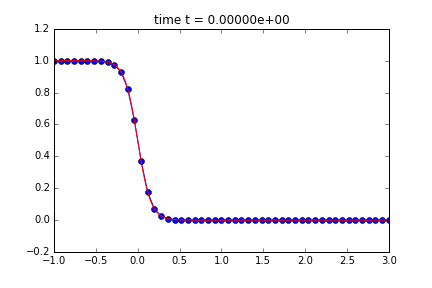
\includegraphics[width=2.8in]{figs/t0.png}\hfil
\hfil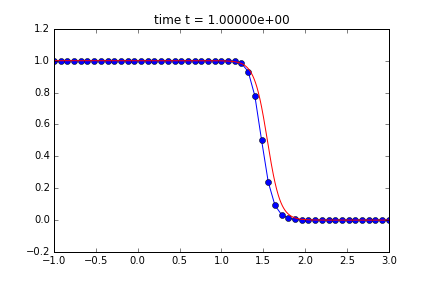
\includegraphics[width=2.8in]{figs/t1.png}\hfil


What order of accuracy do you observe for each choice of ODE solver?
Is it worth using the Runge-Kutta method in view of the first-order errors
introduced by the fractional step method?


% uncomment the next two lines if you want to insert solution...
%\vskip 1cm
%{\bf Solution:}

% insert your solution here!


%--------------------------------------------------------------------------
\vskip 1cm
\hrule
{\bf Extra Credit.}  Worth up to 10 additional points.

Explore what happens
with smaller values of $\epsilon$ and comment on the various
things that can go wrong if the mesh width $h$ and/or the time step $k$ are
not chosen small enough.  Analyze what you see as much as possible.

Some ideas to consider are below, but this is open-ended.
\begin{itemize} 
\item What general guidelines can you deduce from experiments about how $h$
and $k$ should be chosen relative to $\epsilon$ to get good results?

\item Do you think the ODE solver part of this problem is ``stiff'', and
would you be able to take larger time steps if you replaced the explicit
solver by an implicit method such as TR-BDF2?  

\item If you try using an implicit method and take much larger time steps (e.g.
with $k/\epsilon \gg 1$), what sort of behavior do you see, and why?

\item Would it be better to use TR-BDF2 in place of Crank-Nicolson for the
diffusion equation?
\end{itemize}  


% uncomment the next two lines if you want to insert solution...
%\vskip 1cm
%{\bf Solution:}

% insert your solution here!


\end{document}

